\documentclass[11pt,a4paper]{article}

% Packages
\usepackage[margin=1in]{geometry}
\usepackage{amsmath}
\usepackage{amssymb}
\usepackage{graphicx}
\usepackage{tikz}
\usepackage{pgfplots}
\usepackage{listings}
\usepackage{xcolor}
\usepackage{hyperref}
\usepackage{fancyhdr}
\usepackage{tcolorbox}
\usepackage{booktabs}

\usetikzlibrary{shapes,arrows,positioning,calc}
\pgfplotsset{compat=1.18}

% Page styling
\setlength{\headheight}{14pt}
\pagestyle{fancy}
\fancyhf{}
\rhead{PID Control Theory}
\lhead{STAR ESP32 Firmware}
\rfoot{\thepage}

% Title
\title{\textbf{PID Control Theory and Implementation}\\
\large ESP32 Motor Control Application}
\author{STAR Firmware Documentation}
\date{\today}

% Code listing style
\lstset{
  language=C,
  basicstyle=\ttfamily\small,
  keywordstyle=\color{blue},
  commentstyle=\color{gray},
  stringstyle=\color{red},
  showstringspaces=false,
  breaklines=true,
  frame=single,
  numbers=left,
  numberstyle=\tiny\color{gray}
}

\begin{document}

\maketitle
\tableofcontents
\newpage

\section{Introduction}

A PID (Proportional-Integral-Derivative) controller is a feedback control mechanism widely used in industrial control systems. In the context of ESP32-based motor control, PID controllers enable precise closed-loop control by continuously calculating an error value as the difference between a desired setpoint and a measured process variable.

\subsection{Control System Overview}

The STAR firmware implements a discrete-time PID controller specifically designed for:
\begin{itemize}
  \item Brushed DC motor speed control
  \item Position control with encoder feedback
  \item Temperature-compensated motor drive systems
  \item Battery-powered robotic applications
\end{itemize}

\section{Mathematical Foundation}

\subsection{Continuous-Time PID Equation}

The ideal continuous-time PID controller is defined by:

\begin{tcolorbox}[colback=blue!5!white,colframe=blue!75!black,title=Continuous PID Equation]
\begin{equation}
u(t) = K_p e(t) + K_i \int_0^t e(\tau) d\tau + K_d \frac{de(t)}{dt}
\end{equation}
\end{tcolorbox}

where:
\begin{itemize}
  \item $u(t)$ = control output (e.g., motor PWM duty cycle)
  \item $e(t) = r(t) - y(t)$ = error signal
  \item $r(t)$ = setpoint (desired value)
  \item $y(t)$ = measured process variable (actual value)
  \item $K_p$ = proportional gain
  \item $K_i$ = integral gain
  \item $K_d$ = derivative gain
\end{itemize}

\subsection{Discrete-Time Implementation}

For digital implementation on a microcontroller, the PID equation is discretized using numerical approximation:

\begin{tcolorbox}[colback=green!5!white,colframe=green!75!black,title=Discrete PID Equation]
\begin{equation}
u[k] = K_p e[k] + K_i \sum_{j=0}^{k} e[j] \Delta t + K_d \frac{e[k] - e[k-1]}{\Delta t}
\end{equation}
\end{tcolorbox}

where:
\begin{itemize}
  \item $k$ = discrete time step index
  \item $\Delta t$ = sampling period (e.g., 0.001s for 1000Hz control loop)
  \item $e[k] = r[k] - y[k]$ = error at time step $k$
\end{itemize}

\subsection{Component Analysis}

\subsubsection{Proportional Term}

\begin{equation}
P[k] = K_p e[k]
\end{equation}

\textbf{Effect:} Provides immediate corrective action proportional to the current error. Higher $K_p$ increases system responsiveness but may cause overshoot and oscillation.

\subsubsection{Integral Term}

\begin{equation}
I[k] = K_i \sum_{j=0}^{k} e[j] \Delta t = K_i \left( I[k-1] + e[k] \Delta t \right)
\end{equation}

\textbf{Effect:} Eliminates steady-state error by accumulating past errors. Higher $K_i$ speeds up steady-state convergence but may cause overshoot and instability.

\textbf{Anti-Windup:} The integral term is clamped to prevent excessive accumulation:
\begin{equation}
I[k] = \text{clamp}(I[k], I_{\min}, I_{\max})
\end{equation}

\subsubsection{Derivative Term}

\begin{equation}
D[k] = K_d \frac{e[k] - e[k-1]}{\Delta t}
\end{equation}

\textbf{Effect:} Provides damping by predicting future error based on rate of change. Reduces overshoot and improves stability, but is sensitive to noise.

\section{Block Diagram}

\begin{figure}[h]
\centering
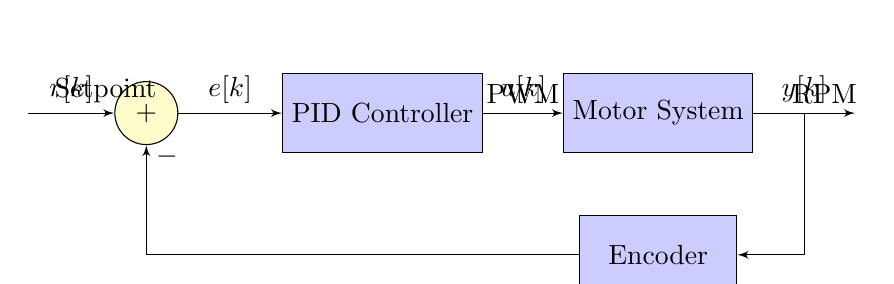
\begin{tikzpicture}[auto, node distance=2cm,>=latex']
  % Styles
  \tikzstyle{block} = [draw, rectangle, minimum height=1cm, minimum width=2cm, fill=blue!20]
  \tikzstyle{sum} = [draw, circle, node distance=1.5cm, minimum size=0.8cm, fill=yellow!20]
  \tikzstyle{input} = [coordinate]
  \tikzstyle{output} = [coordinate]

  % Nodes
  \node [input] (input) {};
  \node [sum, right of=input] (sum) {$+$};
  \node [block, right of=sum, node distance=3cm] (controller) {PID Controller};
  \node [block, right of=controller, node distance=3.5cm] (plant) {Motor System};
  \node [output, right of=plant, node distance=2.5cm] (output) {};
  \node [block, below of=plant, node distance=1.8cm] (sensor) {Encoder};

  % Connections
  \draw [->] (input) -- node {$r[k]$} node[pos=0.9, above] {Setpoint} (sum);
  \draw [->] (sum) -- node {$e[k]$} (controller);
  \draw [->] (controller) -- node {$u[k]$} node[pos=0.5, above] {PWM} (plant);
  \draw [->] (plant) -- node [name=y] {$y[k]$} node[pos=0.7, above] {RPM} (output);
  \draw [->] (y) |- (sensor);
  \draw [->] (sensor) -| node[pos=0.95, right] {$-$} (sum);

\end{tikzpicture}
\caption{Closed-Loop PID Control System Block Diagram}
\label{fig:block_diagram}
\end{figure}

The control loop operates as follows:
\begin{enumerate}
  \item \textbf{Error Calculation:} $e[k] = r[k] - y[k]$
  \item \textbf{PID Computation:} Calculate $P$, $I$, $D$ terms
  \item \textbf{Output Generation:} $u[k] = P[k] + I[k] + D[k]$
  \item \textbf{Actuation:} Apply $u[k]$ to motor (PWM duty cycle)
  \item \textbf{Measurement:} Read encoder position/velocity
  \item \textbf{Feedback:} Use $y[k]$ for next iteration
\end{enumerate}

\section{PID Control Flow}

\begin{figure}[h]
\centering
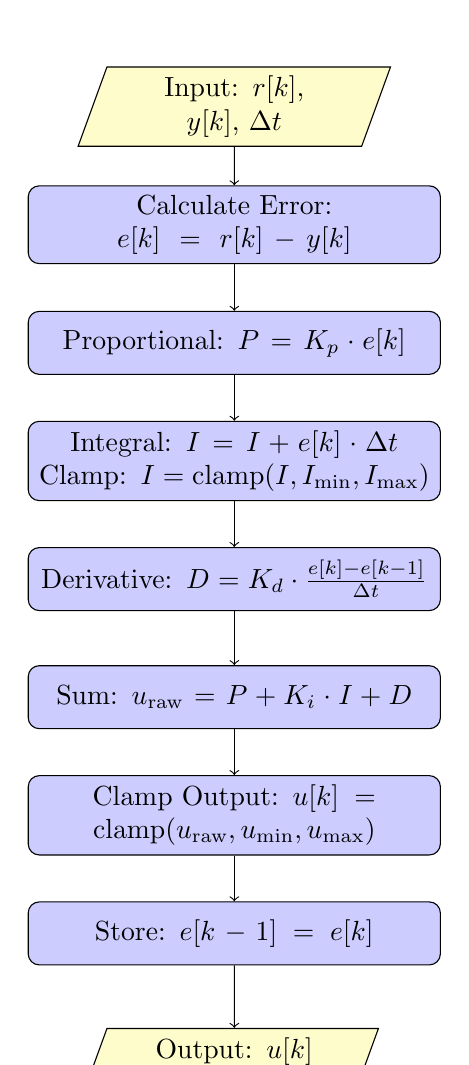
\begin{tikzpicture}[node distance=1.5cm]
  \tikzstyle{process} = [rectangle, draw, fill=blue!20, text width=5cm, text centered, rounded corners, minimum height=0.8cm]
  \tikzstyle{decision} = [diamond, draw, fill=green!20, text width=3cm, text centered, minimum height=1cm]
  \tikzstyle{data} = [trapezium, trapezium left angle=70, trapezium right angle=110, draw, fill=yellow!20, text width=3cm, text centered]

  \node [data] (input) {Input: $r[k]$, $y[k]$, $\Delta t$};
  \node [process, below of=input] (error) {Calculate Error: $e[k] = r[k] - y[k]$};
  \node [process, below of=error] (p) {Proportional: $P = K_p \cdot e[k]$};
  \node [process, below of=p] (i) {Integral: $I = I + e[k] \cdot \Delta t$\\Clamp: $I = \text{clamp}(I, I_{\min}, I_{\max})$};
  \node [process, below of=i] (d) {Derivative: $D = K_d \cdot \frac{e[k] - e[k-1]}{\Delta t}$};
  \node [process, below of=d] (sum) {Sum: $u_{\text{raw}} = P + K_i \cdot I + D$};
  \node [process, below of=sum] (clamp) {Clamp Output: $u[k] = \text{clamp}(u_{\text{raw}}, u_{\min}, u_{\max})$};
  \node [process, below of=clamp] (store) {Store: $e[k-1] = e[k]$};
  \node [data, below of=store] (output) {Output: $u[k]$};

  \draw [->] (input) -- (error);
  \draw [->] (error) -- (p);
  \draw [->] (p) -- (i);
  \draw [->] (i) -- (d);
  \draw [->] (d) -- (sum);
  \draw [->] (sum) -- (clamp);
  \draw [->] (clamp) -- (store);
  \draw [->] (store) -- (output);
\end{tikzpicture}
\caption{PID Algorithm Execution Flow}
\label{fig:flow_diagram}
\end{figure}

\newpage

\section{ESP32 Implementation Details}

\subsection{Data Structures}

The STAR firmware uses two primary structures:

\begin{lstlisting}
// Configuration structure (initialization)
typedef struct {
  float kp;            // Proportional gain
  float ki;            // Integral gain
  float kd;            // Derivative gain
  float output_min;    // Minimum output limit
  float output_max;    // Maximum output limit
  float integral_min;  // Anti-windup lower limit
  float integral_max;  // Anti-windup upper limit
} star_pid_config_t;

// Runtime handle (state preservation)
typedef struct {
  float kp, ki, kd;           // PID gains
  float output_min, output_max;
  float integral_min, integral_max;
  float integral;             // Accumulated integral
  float prev_error;          // Previous error (for derivative)
  bool initialized;          // Initialization flag
} star_pid_handle_t;
\end{lstlisting}

\subsection{Initialization}

\begin{lstlisting}
star_pid_handle_t pid;
star_pid_config_t config = {
    .kp = 1.0f,
    .ki = 0.5f,
    .kd = 0.1f,
    .output_min = -100.0f,  // -100% duty cycle
    .output_max = 100.0f,   // +100% duty cycle
    .integral_min = -50.0f,
    .integral_max = 50.0f,
};
esp_err_t ret = star_pid_init(&pid, &config);
\end{lstlisting}

\subsection{Control Loop Execution}

Typical execution at 1000Hz (1ms sampling period):

\begin{lstlisting}
float setpoint_rpm = 100.0f;
float measured_rpm = 95.0f;
float dt = 0.001f;  // 1ms

float output;
star_pid_compute(&pid, setpoint_rpm, measured_rpm, dt, &output);

// Apply output to motor driver
star_drv8243_set_speed(&motor, output);
\end{lstlisting}

\section{Anti-Windup Mechanism}

\subsection{The Windup Problem}

Integral windup occurs when the control output saturates (reaches $u_{\min}$ or $u_{\max}$) but the error remains non-zero. The integral term continues accumulating, leading to:
\begin{itemize}
  \item Large overshoot when error changes sign
  \item Slow recovery from saturation
  \item System instability
\end{itemize}

\subsection{Clamping Solution}

The STAR implementation uses \textbf{integral clamping}:

\begin{equation}
I[k] = \begin{cases}
I_{\max} & \text{if } I[k] > I_{\max} \\
I_{\min} & \text{if } I[k] < I_{\min} \\
I[k] & \text{otherwise}
\end{cases}
\end{equation}

This prevents the integral term from accumulating beyond practical limits, ensuring:
\begin{itemize}
  \item Bounded integral accumulation
  \item Faster recovery from saturation
  \item Predictable transient response
\end{itemize}

\begin{figure}[h]
\centering
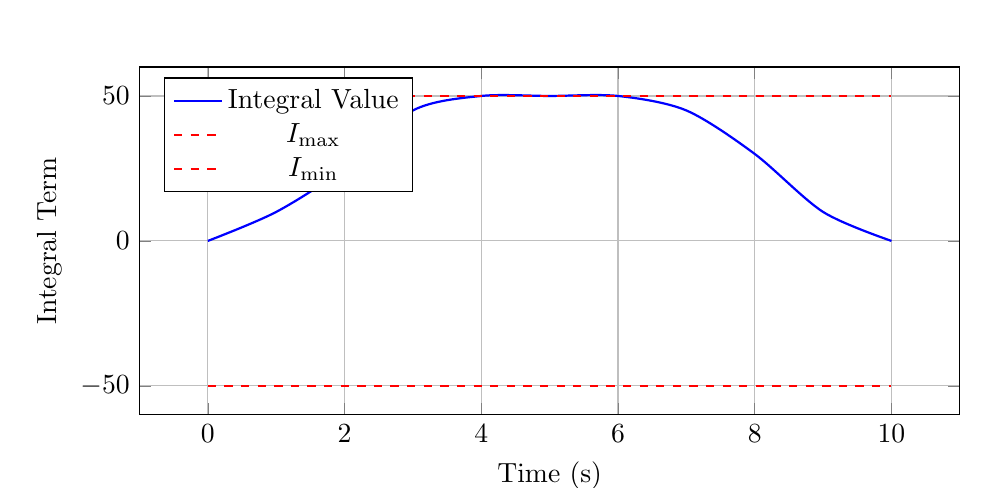
\begin{tikzpicture}
  \begin{axis}[
    width=12cm,
    height=6cm,
    xlabel={Time (s)},
    ylabel={Integral Term},
    grid=major,
    legend pos=north west,
    ymin=-60, ymax=60
  ]
  \addplot[blue, thick, smooth] coordinates {
    (0,0) (1,10) (2,25) (3,45) (4,50) (5,50) (6,50) (7,45) (8,30) (9,10) (10,0)
  };
  \addplot[red, dashed, thick] coordinates {(0,50) (10,50)};
  \addplot[red, dashed, thick] coordinates {(0,-50) (10,-50)};
  \legend{Integral Value, $I_{\max}$, $I_{\min}$}
  \end{axis}
\end{tikzpicture}
\caption{Integral Clamping Prevents Windup}
\end{figure}

\section{Tuning Guidelines}

\subsection{Ziegler-Nichols Method}

A classical tuning approach:

\begin{enumerate}
  \item Set $K_i = K_d = 0$
  \item Increase $K_p$ until system oscillates
  \item Record ultimate gain $K_u$ and oscillation period $T_u$
  \item Calculate gains:
\end{enumerate}

\begin{table}[h]
\centering
\begin{tabular}{lccc}
\toprule
\textbf{Controller} & $K_p$ & $K_i$ & $K_d$ \\
\midrule
P & $0.5 K_u$ & - & - \\
PI & $0.45 K_u$ & $1.2 K_p / T_u$ & - \\
PID & $0.6 K_u$ & $2 K_p / T_u$ & $K_p T_u / 8$ \\
\bottomrule
\end{tabular}
\caption{Ziegler-Nichols Tuning Parameters}
\end{table}

\subsection{Manual Tuning Process}

\begin{enumerate}
  \item \textbf{Start with P-only:} Set $K_i = K_d = 0$, increase $K_p$ until acceptable response
  \item \textbf{Add Integral:} Increase $K_i$ to eliminate steady-state error
  \item \textbf{Add Derivative:} Increase $K_d$ to reduce overshoot and improve stability
  \item \textbf{Fine-tune:} Adjust all three gains iteratively
\end{enumerate}

\subsection{Gain Effects Summary}

\begin{table}[h]
\centering
\begin{tabular}{lccc}
\toprule
\textbf{Parameter} & \textbf{Rise Time} & \textbf{Overshoot} & \textbf{Steady-State Error} \\
\midrule
$K_p \uparrow$ & Decrease & Increase & Decrease \\
$K_i \uparrow$ & Decrease & Increase & Eliminate \\
$K_d \uparrow$ & Minor change & Decrease & No effect \\
\bottomrule
\end{tabular}
\caption{Effect of Increasing PID Gains}
\end{table}

\section{Performance Characteristics}

\subsection{Stability Criteria}

For a stable closed-loop system:

\begin{equation}
\text{Phase Margin} > 45^\circ \quad \text{and} \quad \text{Gain Margin} > 6 \text{ dB}
\end{equation}

\subsection{Step Response Specifications}

\begin{itemize}
  \item \textbf{Rise Time ($t_r$):} Time to reach 90\% of setpoint
  \item \textbf{Settling Time ($t_s$):} Time to stay within $\pm 2\%$ of setpoint
  \item \textbf{Overshoot ($M_p$):} $M_p = \frac{y_{\max} - y_{\text{ss}}}{y_{\text{ss}}} \times 100\%$
  \item \textbf{Steady-State Error ($e_{ss}$):} $e_{ss} = \lim_{t \to \infty} |r(t) - y(t)|$
\end{itemize}

\begin{figure}[h]
\centering
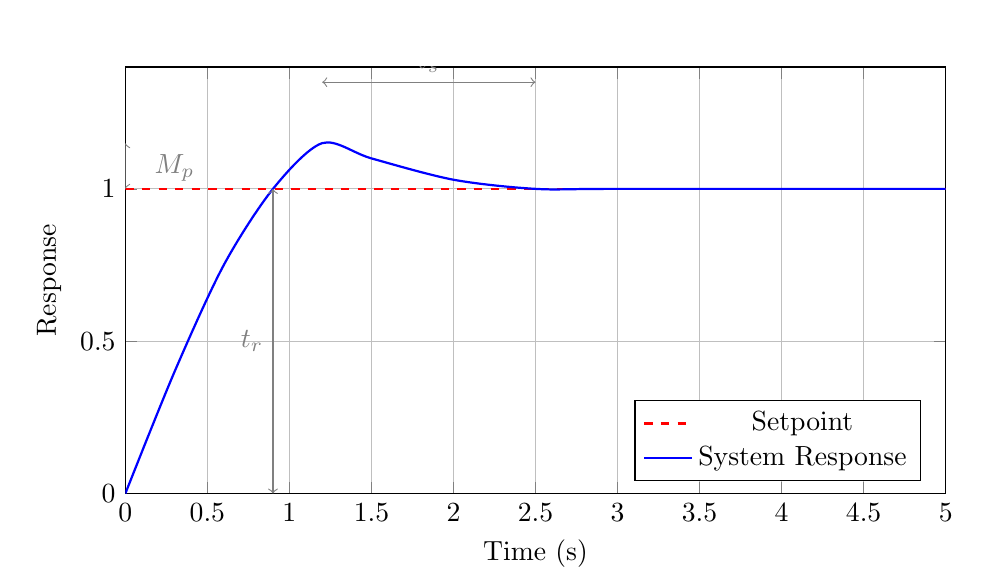
\begin{tikzpicture}
  \begin{axis}[
    width=12cm,
    height=7cm,
    xlabel={Time (s)},
    ylabel={Response},
    grid=major,
    legend pos=south east,
    ymin=0, ymax=1.4,
    xmin=0, xmax=5
  ]
  \addplot[red, dashed, thick] coordinates {(0,1) (5,1)};
  \addplot[blue, thick, smooth] coordinates {
    (0,0) (0.3,0.4) (0.6,0.75) (0.9,1.0) (1.2,1.15) (1.5,1.1) (2.0,1.03) (2.5,1.0) (3,1.0) (5,1.0)
  };
  \draw[<->, gray] (0.9,0) -- (0.9,1.0);
  \node[gray] at (0.9,0.5) [left] {$t_r$};
  \draw[<->, gray] (0,1.0) -- (0,1.15);
  \node[gray] at (0.3,1.07) {$M_p$};
  \draw[<->, gray] (1.2,1.35) -- (2.5,1.35);
  \node[gray] at (1.85,1.35) [above] {$t_s$};
  \legend{Setpoint, System Response}
  \end{axis}
\end{tikzpicture}
\caption{Typical Step Response Characteristics}
\end{figure}

\section{Motor Control Application}

\subsection{Complete System Example}

\begin{lstlisting}
// Initialize motor driver (DRV8243)
star_drv8243_handle_t motor;
star_drv8243_config_t motor_cfg = {
    .bus_manager = &bus_manager,
    .pin_pwm_ph = GPIO_NUM_25,
    .pwm_freq_hz = 20000,  // 20 kHz PWM
};
star_drv8243_init(&motor, &motor_cfg);

// Initialize encoder
star_encoder_handle_t encoder;
star_encoder_config_t enc_cfg = {
    .pcnt_unit = PCNT_UNIT_0,
    .pin_a = GPIO_NUM_32,
    .pin_b = GPIO_NUM_33,
};
star_encoder_init(&encoder, &enc_cfg);

// Initialize PID
star_pid_handle_t pid;
star_pid_config_t pid_cfg = {
    .kp = 1.0f, .ki = 0.5f, .kd = 0.1f,
    .output_min = -100.0f, .output_max = 100.0f,
};
star_pid_init(&pid, &pid_cfg);

// Control loop (1000Hz)
while (1) {
    float velocity_rpm;
    star_encoder_get_velocity_rpm(&encoder, 1.0f, 500, &velocity_rpm);

    float output;
    star_pid_compute(&pid, 100.0f, velocity_rpm, 0.001f, &output);
    star_drv8243_set_speed(&motor, output);

    vTaskDelay(pdMS_TO_TICKS(1));
}
\end{lstlisting}

\section{Advanced Topics}

\subsection{Derivative Filtering}

To reduce noise sensitivity, the derivative term can be filtered:

\begin{equation}
D_{\text{filtered}}[k] = \alpha D[k] + (1 - \alpha) D_{\text{filtered}}[k-1]
\end{equation}

where $\alpha \in [0, 1]$ is the filter coefficient.

\subsection{Feed-Forward Control}

For improved tracking performance, add feed-forward term:

\begin{equation}
u[k] = u_{\text{PID}}[k] + K_{ff} r[k]
\end{equation}

\subsection{Bumpless Transfer}

When switching between manual and automatic mode, initialize integral term:

\begin{equation}
I[k] = \frac{u_{\text{manual}} - P[k] - D[k]}{K_i}
\end{equation}

\section{References}

\begin{enumerate}
  \item Astrom, K. J., \& Hagglund, T. (2006). \textit{Advanced PID Control}. ISA.
  \item Franklin, G. F., Powell, J. D., \& Emami-Naeini, A. (2019). \textit{Feedback Control of Dynamic Systems} (8th ed.). Pearson.
  \item ESP-IDF Documentation: Motor Control Peripheral (MCPWM)
  \item STAR Firmware Documentation: \texttt{lib/star\_pid/}
\end{enumerate}

\appendix

\section{Implementation Source Code}

\subsection{PID Compute Function}

\begin{lstlisting}
esp_err_t star_pid_compute(star_pid_handle_t* handle,
                            float setpoint,
                            float measured,
                            float dt,
                            float* output)
{
  // Validate inputs
  if (!handle || !output || dt <= 0.0f) {
    return ESP_ERR_INVALID_ARG;
  }

  // Calculate error
  float error = setpoint - measured;

  // Proportional term
  float p_term = handle->kp * error;

  // Integral term with anti-windup
  handle->integral += error * dt;
  handle->integral = clamp(handle->integral,
                           handle->integral_min,
                           handle->integral_max);
  float i_term = handle->ki * handle->integral;

  // Derivative term
  float derivative = (error - handle->prev_error) / dt;
  float d_term = handle->kd * derivative;

  // Compute total output
  float raw_output = p_term + i_term + d_term;

  // Clamp output to limits
  *output = clamp(raw_output,
                  handle->output_min,
                  handle->output_max);

  // Store error for next iteration
  handle->prev_error = error;

  return ESP_OK;
}
\end{lstlisting}

\section{Typical Parameter Ranges}

\begin{table}[h]
\centering
\begin{tabular}{lll}
\toprule
\textbf{Parameter} & \textbf{Typical Range} & \textbf{Motor Control Application} \\
\midrule
$K_p$ & 0.1 - 10.0 & 0.5 - 2.0 (velocity control) \\
$K_i$ & 0.01 - 5.0 & 0.1 - 1.0 (eliminate steady-state error) \\
$K_d$ & 0.001 - 1.0 & 0.01 - 0.2 (damping) \\
$\Delta t$ & 0.001 - 0.1 s & 0.001 s (1000 Hz recommended) \\
Output Limits & System-dependent & $\pm 100$ (PWM duty cycle \%) \\
Integral Limits & 50-100\% of output & $\pm 50$ (anti-windup) \\
\bottomrule
\end{tabular}
\caption{Typical PID Parameter Ranges}
\end{table}

\end{document}
